\chapter{Requirements}
\label{cha:requirements}

This  work deals  with  an  execution environment  that  uses Xen  virtual
machines to run  applications in a secure environment.   In this chapter I
am going to describe, how such an environment can look like and what it is
supposed to provide the users with.

\begin{figure}[htbp]
  \centering
  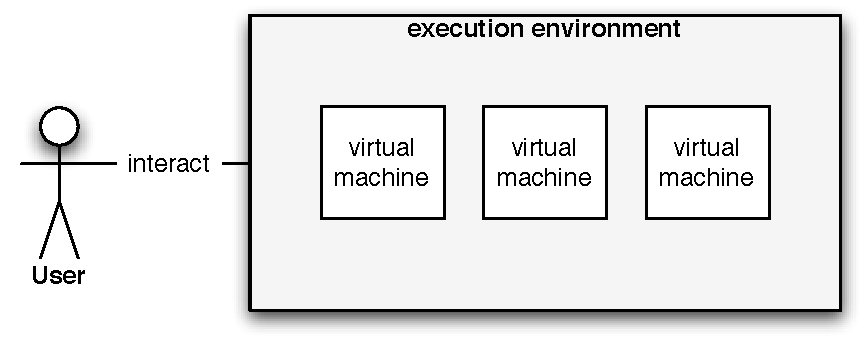
\includegraphics[scale=.5]{concept}
  \caption[Conceptual overview]{A conceptual overview}
  \label{fig:concept}
\end{figure}

In Figure~\ref{fig:concept},  a conceptual overview  is shown, it  depicts a
single user interacting with the execution environment.

The next sections describe what  I think, an execution environment must at
least provide to be useful. Furthermore, several use-cases are given, that
show possible usage scenarios of the execution environment.

\section{Execution environment}
\label{sec:req-execution-environment}

What should an execution environment  provide, so that users can work with
it?  I  think  the following  list  gives  a  good  idea about  the  basic
requirements any execution environment should fulfill:

\begin{itemize}
\item \emph{Submit new tasks} --- i.e.~inform the system about a new task,
  that it should execute.
\item \emph{Query the status of  tasks} --- i.e.~is the task still pending
  and  waiting for  its execution,  currently  running or  did it  already
  finish.
\item \emph{Stop running tasks} --- i.e.~a user must always have the
  possibility to cancel his own tasks.
\end{itemize}

Typically, tasks  require some input data  to work on  and generate output
data  ---  to describe  such  tasks  we  demand the  following  additional
requirements:
\begin{itemize}
\item Provide a way to specify input data for a task
\item Provide a way to retrieve generated output data from a task
\end{itemize}

The next sections describe each point in more detail --- they also explain
specifications  such  as the  \emph{Job  Submission Description  Language}
(\gls{glo:JSDL}) \cite{jsdl-spec}  and the \emph{Basic  Execution Service}
(\gls{glo:BES}) \cite{ogsa-bes}.

\subsection{Submission of tasks}
\label{sec:req-task-submission}

In  grid environments,  for example,  the user  describes his  job  as the
application he wants to execute,  additional parameters that are passed to
the application, input and output data and many more.

The here proposed execution environment demands a way to describe not only
the tasks, but also  the virtual machine that is going to  be used for the
task.

An upcoming standard for a job description, that is not restricted to grid
environments, but  can be used  in various environments, is  the \emph{Job
  Submission  Description  Language}   ---  or  \gls{glo:JSDL}  for  short
\cite{jsdl-spec}.

I  decided to  use this  description language,  so that  the Xen-execution
environment can  easily be integrated  into various middlewares  that also
use the \gls{glo:JSDL} to describe their jobs.


\subsubsection{Extensions to the \gls{glo:JSDL}}

To be able to create a virtual machine on the remote site, the user has to
specify not only  the application she wants to run  but also a file-system
\gls{glo:image}  that  contains  an  operating system  installation.   The
execution environment then  takes care of starting up  the virtual machine
with  the  provided  \gls{glo:image}   and  will  eventually  execute  the
application.

The  description  of a  virtual  machine cannot  be  done  using only  the
\gls{glo:JSDL},  since one has  to describe  additional locations  for the
\gls{glo:image}, a  kernel and probably an initial  RAM-disk.  Those files
are not directly  related to the description of a job  and one cannot just
use  \texttt{DataStaging}  elements, since  they  act  on the  file-system
hierarchy seen from the job's  point of view, i.e.~from within the virtual
machine.   The extensions  made  to the  \gls{glo:JSDL}  are discussed  in
chapter \ref{cha:design} in more detail.

\subsection{Query the status of tasks}
\label{sec:status-query}

A user  who submitted a task  to some remote system  for execution, surely
wants to observe the current state of his job. The query for the status of
a   job  requires  the   detailed  specification   of  which   states  are
\textbf{allowed  states}  and  how  the \textbf{transitions}  between  the
states look like.

To provide  the possibility to connect the  Xen-execution environment with
other  tools,  a  common  description  for job-states  is  required.   The
\emph{Open Grid Services Architecture} (\gls{glo:OGSA}, \cite{ogsa}) has a
working group which designs such a common state model for job execution in
grid environments  --- the \emph{Basic  Execution Service} (\gls{glo:BES},
\cite{ogsa-bes}).

The OGSA is an approach to  use Web service concepts and technologies in a
Grid  environment. Consequently, the BES defines a Web service, but I will
just make use of the generic job-state-model they define.

\subsubsection{Extensions to the BES state-model}

Since the basic  \gls{glo:BES} state-model is a very  minimal one, we need
to  extend   it  to  allow   the  description  of   data-transfer  states.
Fortunately,  the \gls{glo:BES}  provides such  an extended  model  in its
specification, it is shown in Figure~\ref{fig:bes-extended}.

\begin{figure}
  \centering
  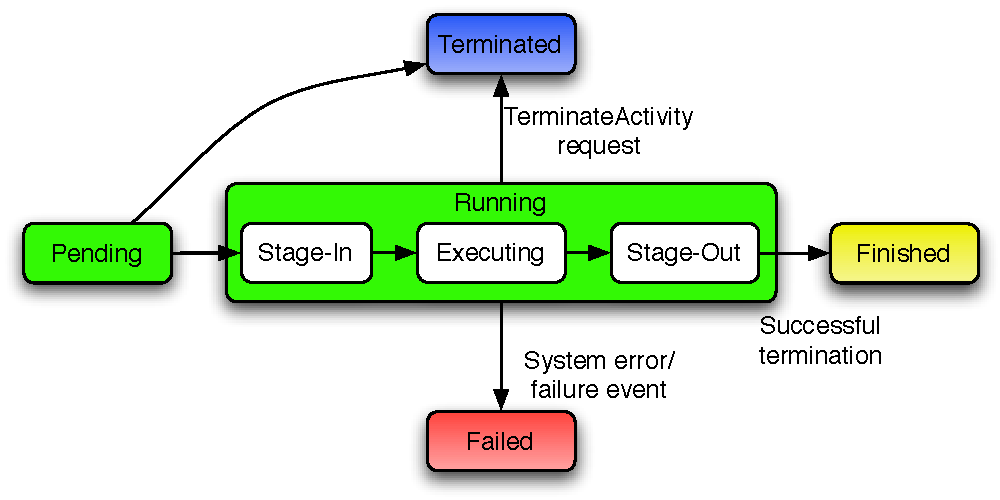
\includegraphics[scale=.75]{bes-staging-job-model}
  \caption[BES State Model Staging Extension]{The basic BES state-model
    extended with sub-states to describe data-transfers.}
  \label{fig:bes-extended}
\end{figure}

The  \texttt{Running}   state  has   been  split  into   three  sub-states
\texttt{Stage-In}, \texttt{Stage-Out} and \texttt{Executing} --- the first
two describe data-transfer operations and the last one describes the state
in which the task is  actually being executed.  An invalid specialization,
for  example,  would   have  been  the  addition  of   a  transition  from
\texttt{Running:Stage-In} back  to \texttt{Pending}, since  that behaviour
is impossible in the basic state-model.

The  \gls{glo:BES}  specification  as  it  is for  the  JSDL,  defines  an
XML-Schema,  that is  to  be  used for  state  description. The  following
example shows  you the usage  of the state  description using XML  and how
specialized sub-states are represented. The main state is \texttt{Running}
and is  described using the \emph{ActivityStatus}  element, any sub-state,
that may currently be active,  depends on the application and therefore is
described using one or more elements from a different namespace.

\begin{minipage}{0.75\textwidth}
  \begin{lstlisting}[language=XML]
    <bes:ActivityStatus state="Running">
       <n00:Stage-In/>
    </bes:ActivityStatus>
  \end{lstlisting}
\end{minipage}

The example  makes use of  the previously defined  specialized state-model
and  describes an  activity  that is  currently  in the  \texttt{Stage-In}
sub-state of \texttt{Running} --- i.e.~it is waiting for its input data to
be  ready.  Any  client  which  is  not  aware  of  the  \texttt{Stage-In}
sub-state, will only ``see'' that  the activity is in the \texttt{Running}
state.


\subsection{Stopping tasks}
\label{sec:stopping-task}

As  you can  see in  Figure~\ref{fig:bes-extended}, each  non-terminal state
provides  a transition  to  the state  \texttt{Terminated}. That  directly
resembles the requirements for \emph{stopping a task} on user request.

In  case of  this work,  stopping  a task  may involve  shutting down  the
virtual  machine,  terminating active  data  transfers  and releasing  any
acquired resources.

\section{A more concrete concept}

This  section   outlines  a  more  concrete  concept   for  the  execution
environment and its  components. We are going to need  a component that is
responsible for  the requests a  user makes to the  execution environment,
this component  is also going to  manage the virtual machines  for each of
the tasks.

\begin{figure}[htbp]
  \centering
  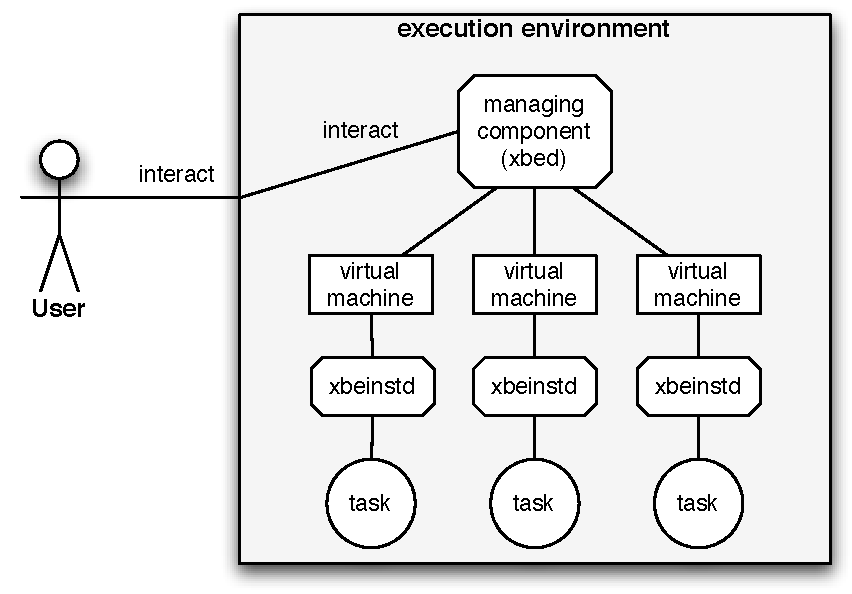
\includegraphics[scale=.5]{concrete-concept}
  \caption[A more concrete concept]{The  evolved concept, using a managing
    component to  control the virtual  machines.  Each virtual  machine is
    dedicated to a single task submitted by some user. Users only interact
    with the managing component.}
  \label{fig:concrete-concept}
\end{figure}

Basically  this concept  defines a  client-server architecture,  where the
client is represented  by the user (or some mediator  such as a web-portal
or a  command-line client) and the  server is represented  by the managing
component.

The following  sections motivate the communication  architecture, which is
used  to connect up  clients and  the managing  component, and  a detailed
description of how the tasks should be handled.

\section{Support for Calana}
\label{sec:calana-support}

To  support  Calana, the  \gls{glo:XenBEE}  must  provide some  additional
functionality. One of these functionalities is a mechanism to \emph{make},
\emph{cancel}   and   \emph{confirm}   reservations.   To   reflect   that
requirement, we discussed about a common state-model for the jobs and came
to the consensus of adopting the \gls{glo:BES} model to our needs.

The implementation of Calana, which is currently still in development, too
uses message queues to implement the communication between the brokers and
the agents.

\begin{figure}[htbp]
  \centering
  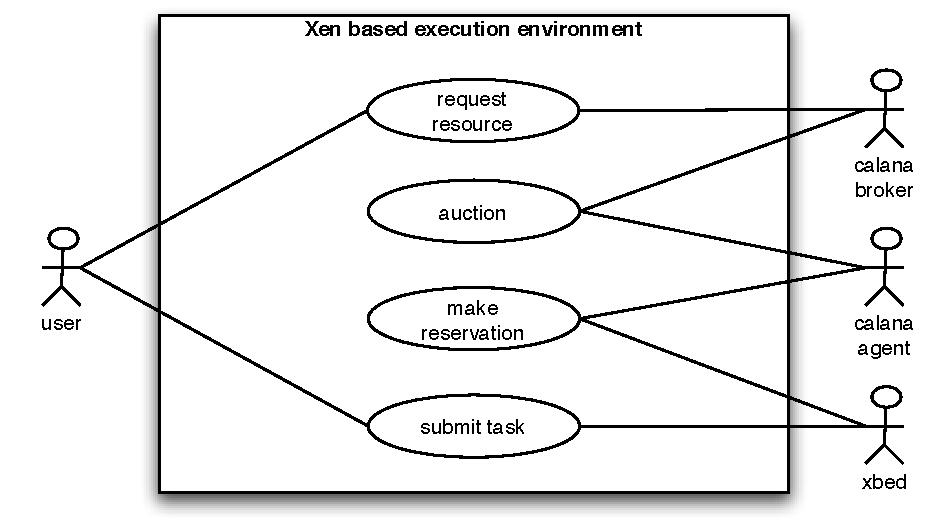
\includegraphics[scale=0.7]{uc-calana-xenbee}
  \caption[Calana and  XenBEE]{The actors and use cases  that are involved
    when a Calana agent uses the \gls{glo:XenBEE} as its resource.}
  \label{fig:calana-xenbee}
\end{figure}

The picture  in Figure~\ref{fig:calana-xenbee} describes how  a user would
interact  with  a  system,  that   uses  Calana  for  scheduling  and  the
\gls{glo:XenBEE} as  its execution environment. The user  first requests a
resource from  the broker, who in turn  will open up an  auction among the
agents.   One of  those  agents are  shown  in the  figure,  he creates  a
reservation on the \emph{xbed} he  is attached to.  The user is eventually
presented  a unique identifier  for his  reservation which  he can  use to
submit his task to the \emph{xbed}.

\section{Use cases}
\label{sec:use-cases}

This section describes possible use cases for the \gls{glo:XenBEE}. I have
already shortly described, what the  basic requirements to this system are
and now  I am  going to show  you some  use cases and  which parts  of the
architecture are involved in each of them.

The ``big picture'' is shown in Figure~\ref{fig:system-usecases}, it shows
a compendium  of several possible  use cases from  a very high  level. The
involved    actors    are     the    \emph{user},    the    \emph{managing
  component}\footnote{denoted as \emph{xbed} --- the ``Xen-based Execution
  Daemon''}     mentioned      earlier     and     a      new     managing
component\footnote{denoted   as   \emph{xbeinstd}   ---  the   ``Xen-based
  Execution Instance Daemon''} which  is running on and solely responsible
for a single virtual machine.

\begin{figure}[htbp]
  \centering
  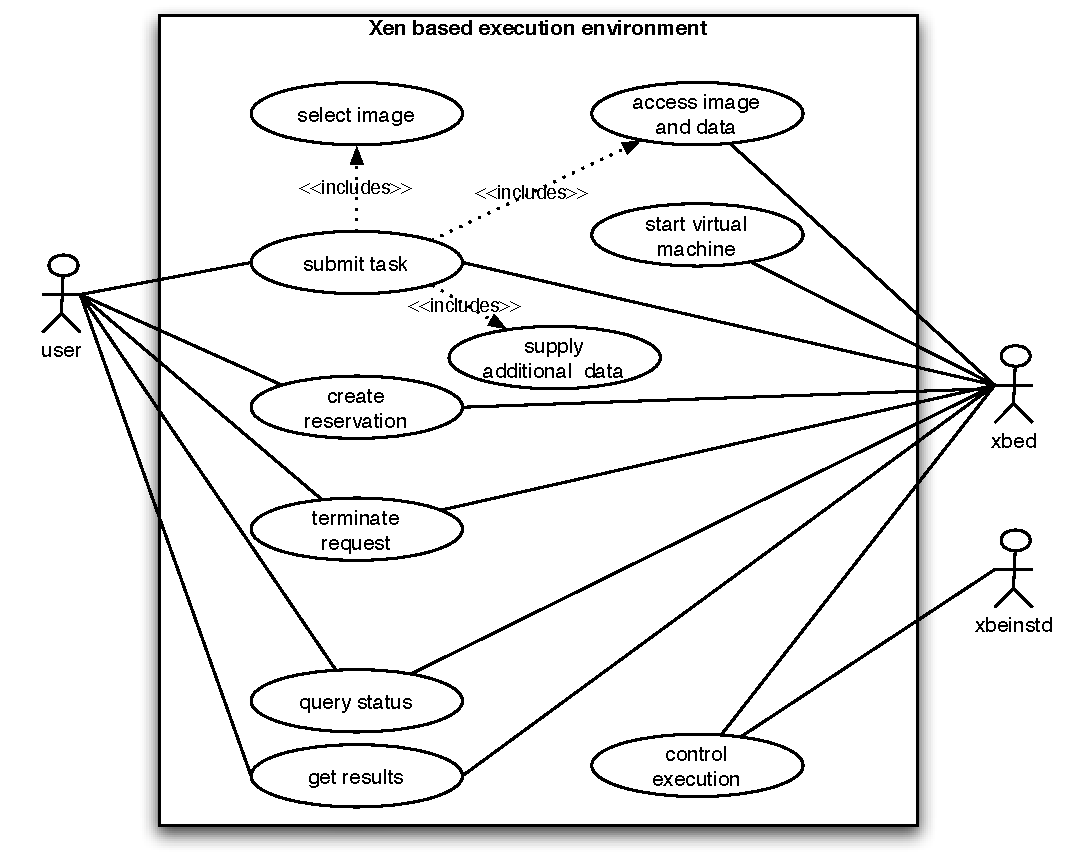
\includegraphics[scale=0.7]{system-usecase}
  \caption[Use case  overview]{An overview  of several possible  use cases
    and the involved actors.}
  \label{fig:system-usecases}
\end{figure}


\subsection{Task submission}
\label{sec:uc-task-submission}

The very  first use case is  the submission of a  \emph{simple} task. With
\emph{simple} I mean, that the  task does not require any additional data,
it just  requires a previously prepared \gls{glo:image}  that contains the
application and the \emph{xbeinstd}.

On  server-side, the  \emph{xbed}  will associate  the  submission with  a
previously acquired  reservation ---  i.e.~the user creates  a reservation
first  which results in  some kind  of handle  (a unique  identifier which
refers to the  reservation) and then the user submits  his task using that
reservation.

\begin{figure}[htbp]
  \centering
  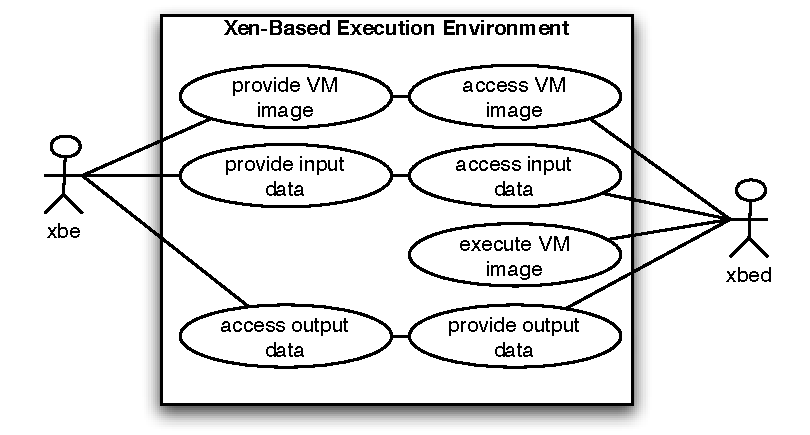
\includegraphics[scale=.75]{uc-submit-task}
  \caption[UC Task submission]{Actors involved  in the task submission use
    case.}
  \label{fig:uc-submit-task}
\end{figure}

\paragraph{Selecting an image}
In  Figure~\ref{fig:uc-submit-task} the  required steps  for  submitting a
task are  shown. The  submission of  a task includes  the selection  of an
image  that  contains  the  application  the user  wants  to  execute.   A
sophisticated process of image-selection  can be rather complicated, since
it involves matching of available images against a description provided by
the user. Such  selection mechanisms are out of the  scope of this thesis,
but  in  a  later  use  case,  server-side  \emph{caching  of  data}  (see
Section~\ref{sec:uc-data-caching}),  a  simple way  of  selection will  be
described.

\paragraph{Accessing the image}
After the user submitted a  task, the \emph{xbed} has to \emph{access} the
specified image,  i.e.~the \emph{xbed} will initiate the  retrieval of the
image.   The  location  of  the  image  can for  example  be  given  as  a
\gls{glo:URI}  to   provide  an  uniform  and   extensible  mechanism  for
describing data locations.

If errors occur  during the image retrieval, the  \emph{xbed} has to abort
the task execution and must inform the user about the failure.

\subsection{Data staging}
\label{sec:uc-data-staging}

This  use case  is an  enhancements  over the  previous one,  it not  only
involves the  submission of an image,  but also the  specification of data
that  must  be  available  prior  executing  the task  and  that  must  be
transfered back to user after the task has finished.

\begin{figure}[htbp]
  \centering
  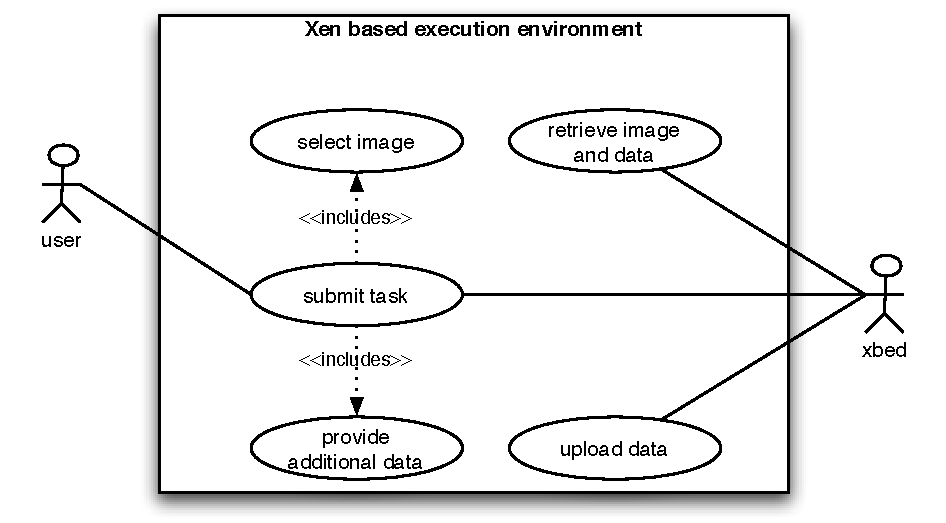
\includegraphics[scale=.75]{uc-data-staging}
  \caption[UC  Data  Staging]{A user  submitting  a  task with  additional
    data.}
  \label{fig:uc-data-staging}
\end{figure}

Again,  the JSDL comes  into play  here, because  it already  supports the
description of staging operations. The \emph{xbed} has now to retrieve not
only  the image  file, but  also  all the  additional files  the user  has
specified to be staged in.

After the job  has finished its execution, the  \emph{xbed} is responsible
for staging  out generated  files. Therefore the  user must  specify which
files that are and to which locations they have to be uploaded. Source and
destination locations of files can again be specified as \gls{glo:URI}s.

\subsection{On-demand VM-deployment}
\label{sec:uc-on-demand-vm-deployment}

Well, this use  case can be seen  as a variant of the  task submission use
case. The purpose of this use case is the creation of a virtual machine on
user request without executing any task.

The resulting virtual  machine could be accessed by  the user through some
remote mechanism such as \gls{glo:SSH} \cite{openssh}.  With \gls{glo:SSH}
the user gains full control over his created virtual machine and can setup
and install any application he likes.

The login  to the  VM can  be provided using  public-keys that  are either
previously  installed  into the  image  or  uploaded  later on  using  the
standard   stage-in   process  (please   consult   the  documentation   on
\gls{glo:SSH} for more information about public-key authorization).


\subsection{Caching of data}
\label{sec:uc-data-caching}

Imagine a user,  who wants to execute the  same application several times.
That would mean he has to submit the same image over and over again, which
imposes a heavy load on the network connecting user and provider (i.e. the
host on which the \emph{xbed} runs). It would be wise to provide a caching
mechanism, that  allows the  user to store  his image on  server-side. The
caching efficiently  reduces network load and  decreases overall execution
time \cite{locality-principle}.

\begin{figure}[h]
  \centering
  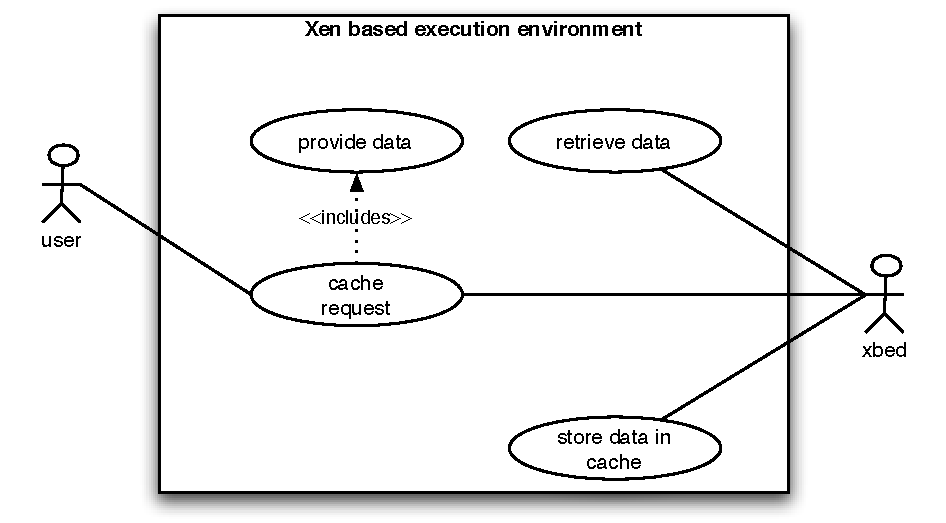
\includegraphics[scale=.75]{uc-data-caching}
  \caption[UC  Data  Caching]{A user  who  is  requesting  the caching  of
    (arbitrary) data.}
  \label{fig:uc-data-caching}
\end{figure}

In  Figure~\ref{fig:uc-data-caching} the required  steps for  caching some
data are  shown. The user  makes his request  for caching the data  to the
\emph{xbed}, which in turn retrieves the data and stores it in a cache. To
make  the ``discovery''  of cached  data easier  for the  users,  the user
should be required to give some descriptive information for the data he is
going to  cache. As the return of  the request, the user  should receive a
unique identifier or an \gls{glo:URI} for the created entry in the cache.

The details  of how  exactly the caching  works are  highly implementation
specific, the most important point is  how the cached data can be referred
to by users of the system at a later point in time.

\paragraph{Referencing cached  data}

Cached data must be referable by the user for subsequent task submissions.
Since the submission of tasks uses \gls{glo:URI}s to indicate the location
of a  file, an obvious  way is  to use a  \gls{glo:URI} here as  well. The
caching of some data should  therefore result in a \gls{glo:URI}, that the
user can use in his job and staging descriptions.

\begin{figure}[h]
  \centering
  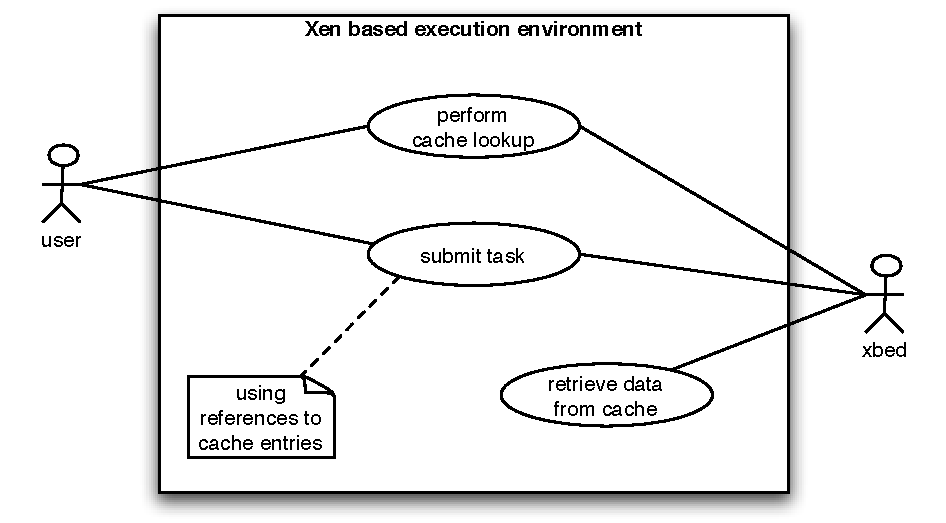
\includegraphics[scale=.75]{uc-cache-lookup}
  \caption[UC  Cache Lookup]{A user  who  is using cached entries within
    his task submission.}
  \label{fig:uc-cache-lookup}
\end{figure}

Additionally, a really  nice thing to have in this  situation is some kind
of a lookup mechanism for cached  entries --- i.e.~a user does not need to
remember all the  \gls{glo:URI}s his entries have, but can  use a query to
the    system   and   thus    figure   out,    which   cache    entry   to
use. Figure~\ref{fig:uc-cache-lookup} shows you  how a user looks up cache
entries and uses them in a subsequent task submission.

\subsection{Terminating a task}
\label{sec:uc-terminate-task}

As   you   could   see   in   the   \gls{glo:BES}   job   state-model   in
Figure~\ref{fig:bes-extended},  the  user  must  have the  possibility  to
terminate his  submitted task at any  time and no matter  what the current
state of the task is.

\begin{figure}[h!]
  \centering
  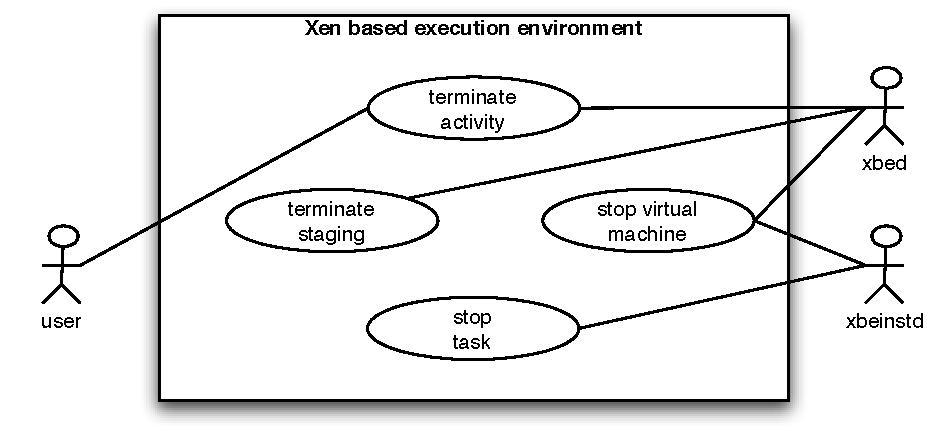
\includegraphics[scale=.75]{uc-terminate-task}
  \caption[UC Terminate Task]{A user  who is requesting the termination of
    his  submitted task  and possible  use cases  that may  then  arise on
    server-side.}
  \label{fig:uc-terminate-task}
\end{figure}

The termination request  for a task can be received in  any state and that
may require  additional actions to be  taken in the  \emph{xbed}.  If, for
instance,  a virtual  machine has  already been  created and  is currently
executing the user's task, the application and the virtual machine have to
be terminated, too.  The same  holds for staging activities, that could be
currently active, they  have to be terminated cleanly  as well.  These use
cases are  shown in  Figure~\ref{fig:uc-terminate-task}. As you  can seen,
the \emph{xbeinstd} may be involved again, since the actual execution of a
task falls within his responsibility.

\subsection{Providing encrypted data}
\label{sec:uc-ecrypted-data}

Since all  data is referred to  by \gls{glo:URI}s, that  may be accessible
not  only  from  the  \emph{xbed}  itself, but  also  from  other  sources
(i.e.~probably unknown and  hostile ones), it is desirable  to store those
files encrypted. Of  course, if a user stores  an encrypted image-file and
wants  the \emph{xbed} to  use it  for execution,  the image-file  must be
decrypted on server-side prior booting a virtual machine with it.

\begin{figure}[h!]
  \centering
  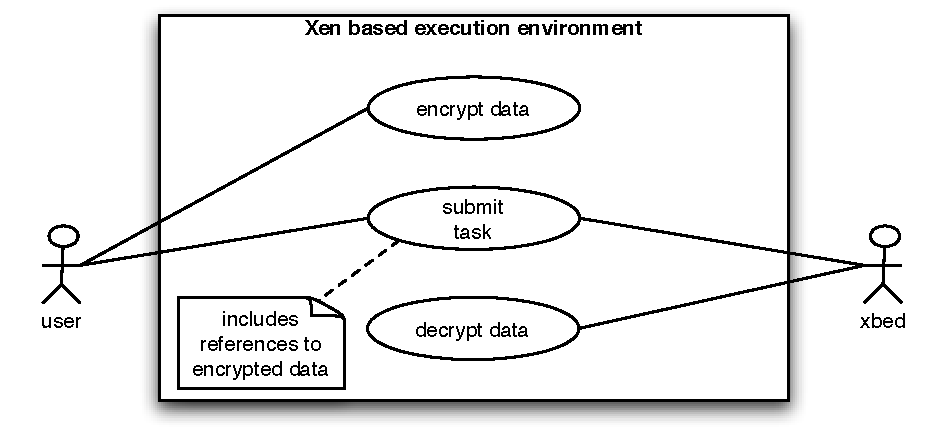
\includegraphics[scale=.75]{uc-encrypted-data}
  \caption[UC  Encrypted  Data]{Submission   of  encrypted  data  and  its
    decryption prior execution by the \emph{xbed}.}
  \label{fig:uc-encrypt-data}
\end{figure}

%%% Local Variables: 
%%% mode: latex
%%% TeX-master: "main.tex"
%%% End: 
